\section{Medical Transformer: Gated Axial-Attention for
Medical Image Segmentation}

\subsection*{Ссылка} \url{https://arxiv.org/abs/2102.10662}
\subsection*{Введение}
Сверточные нейронные сети сравнительно плохо \glqq понимают\grqq зависимости между 
признаками, которые находятся на дальнем расстоянии друг от друга в изображениях. Недавно предложенные 
архитекутры сетей, основанные на трансформерах, используют self-attention механизм для шифрования
дальних зависимостей и выявляют наиболее заметные представления. Эти наблюдения мотивировали авторов 
статьи исследовать решения, в основе которых лежат трансформеры и изучить возможность 
использования архитектур нейронных сетей с трансформерами в задачах медицинской сегментации.

\subsection*{Основная идея}
В данной работе предлагается закрытый, чувствительный к расположению axial attention механизм, который 
хорошо показывает себя на малых наборах данных. Также, вводится эффективная 
методология обучения Local-Global (LoGo)
для трансформеров и Medical-Transformer (MedT) -  метод, построенный на основе двух вышеперечисленных 
предложенных концепций, разработанный специально для сегментации медицинских изображений, который успешно 
улучшает производительность по сравнению со сверточными нейронными сетями и сетями чисто attention архитектуры 
на трех разных датасетах.\\
\begin{minipage}{1.0\linewidth}
    \begin{center}
        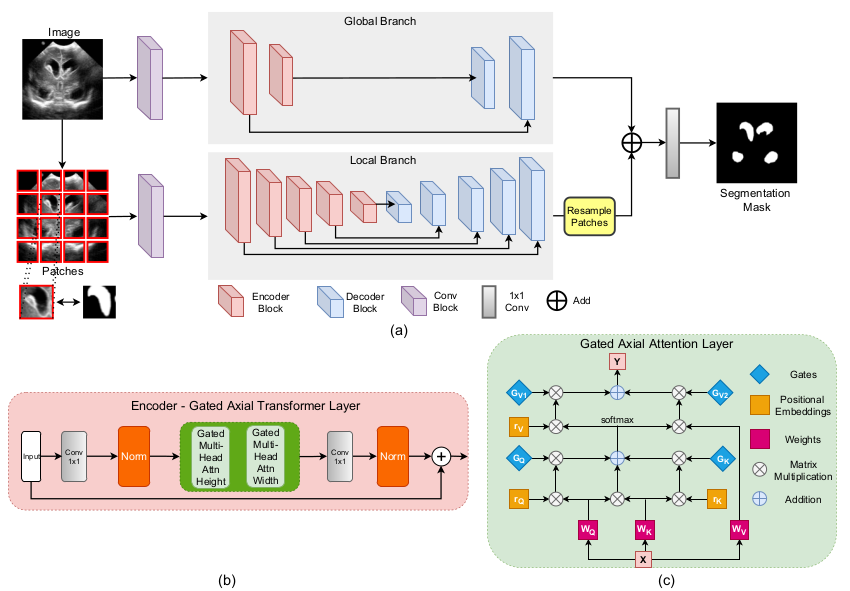
\includegraphics[scale=0.5]{ann18_arch.png} \\
        \caption{\scriptsize{
           Архитектура MedT.
        }}
    \end{center}
    
\end{minipage} 
\subsection*{Данные}
Brain US, Glas, MoNuSeg
\subsection*{Результаты}
\begin{minipage}{1.0\linewidth}
    \begin{center}
        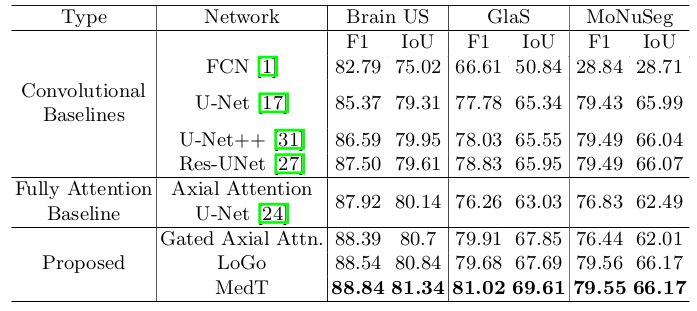
\includegraphics[scale=0.5]{ann18_res.png} \\
        \caption{\scriptsize{
           Количественное сравнение предложенных методов со сверточными бейзлайнами, основанными на трансформерах
           по мерам F1 и IoU.
        }}
    \end{center}
    
\end{minipage} \\

\begin{minipage}{1.0\linewidth}
    \begin{center}
        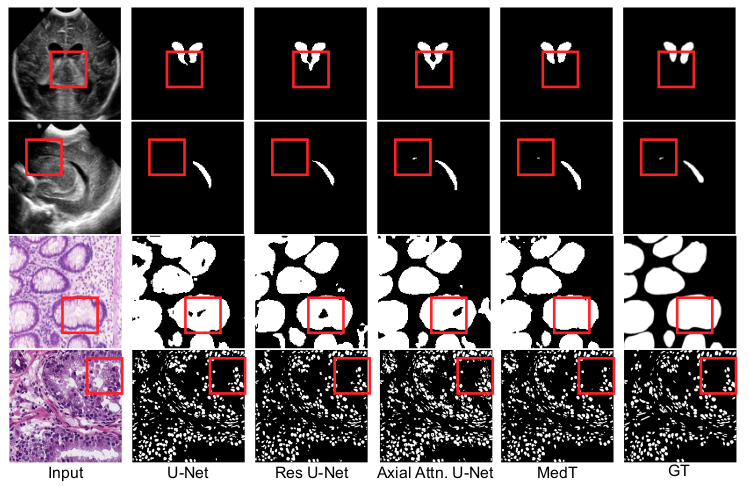
\includegraphics[scale=0.6]{ann18_mri.png} \\
        \caption{\scriptsize{
            Качественные результаты на примерах тестовых изображений из датасетов Brain US, Glas и MoNuSeg.
            Красный прямоугольник очерчивает регионы, где именно MedT показывает лучшие результаты, чем 
            другие методы в сравнении.
        }}
    \end{center}
    
\end{minipage}

\subsection*{Заключение}
В данной статье было продемонстрировано, что предложенные методы превосходят существующие 
в задаче сегментации медицинских изображений не требуя при этом большого набора тренировочных данных.

